% ============================================================
%  يُترجَم بـ XeLaTeX  (في Overleaf: Menu → Compiler → XeLaTeX)
%  الخط: Amiri (متوفر في Overleaf، أو حمّله من github.com/aliftype/amiri)
% ============================================================
\documentclass[12pt,a4paper]{article}
\usepackage[a4paper,margin=1.7cm,top=2.3cm,bottom=2.9cm,headheight=15pt,footskip=1.5cm]{geometry}
\usepackage{amsmath,amssymb}
\usepackage{icomma}
\usepackage[english,bidi=default,layout=lists]{babel}
\babelprovide[import,main]{arabic}
\babelfont{rm}[Scale=1.08]{Amiri}
\babelfont{sf}[Scale=1.08]{Amiri}
\usepackage[most]{tcolorbox}
\usepackage{tikz}
\usetikzlibrary{arrows.meta,calc,shadings}
\usepackage{array}
\usepackage{colortbl}
\usepackage{fancyhdr}
\usepackage{titlesec}
\usepackage{enumitem}
\usepackage{collcell}
\usepackage{needspace}
\usepackage{etoolbox}
\newcolumntype{C}{>{\collectcell\ar}c<{\endcollectcell}}
\pretocmd{\section}{\Needspace{15\baselineskip}}{}{}
\pretocmd{\subsection}{\Needspace{11\baselineskip}}{}{}

\definecolor{cDef}{HTML}{1F4E9C}
\definecolor{cThm}{HTML}{B3261E}
\definecolor{cRem}{HTML}{2E7D32}
\definecolor{cEx}{HTML}{C76B00}
\definecolor{cMeth}{HTML}{6A1B9A}
\definecolor{cSol}{HTML}{00695C}
\definecolor{cSec}{HTML}{1F3A68}

\titleformat{\section}{\Large\bfseries\color{cSec}}{\thesection.}{0.6em}{}[{\color{cSec!60}\titlerule[1pt]}]
\titleformat{\subsection}{\large\bfseries\color{cThm!85!black}}{\thesubsection.}{0.5em}{}
\titlespacing*{\section}{0pt}{14pt}{8pt}
\titlespacing*{\subsection}{0pt}{10pt}{5pt}
\setlength{\parindent}{0pt}
\setlength{\parskip}{4pt}
\setlist{itemsep=2pt,topsep=3pt}

\newtcolorbox{arbox}[3][]{enhanced,
  colback=#2!5,colframe=#2!80!black,arc=2mm,boxrule=0.8pt,
  left=6pt,right=6pt,top=8pt,bottom=5pt,
  fonttitle=\bfseries,coltitle=white,
  title={\foreignlanguage{arabic}{#3}},
  attach boxed title to top right={xshift=-5mm,yshift=-3mm},
  boxed title style={colback=#2!80!black,arc=1.5mm,boxrule=0pt},
  before upper={\selectlanguage{arabic}},
  before skip=8pt,after skip=8pt,breakable,#1}
\newenvironment{BOX}[2]{\begin{otherlanguage}{english}\begin{arbox}{#1}{#2}}{\end{arbox}\end{otherlanguage}}
\newenvironment{tarif}[1][تعريف]{\begin{BOX}{cDef}{#1}}{\end{BOX}}
\newenvironment{khassia}[1][خاصية]{\begin{BOX}{cThm}{#1}}{\end{BOX}}
\newenvironment{molahada}[1][ملاحظة]{\begin{BOX}{cRem}{#1}}{\end{BOX}}
\newenvironment{mithal}[1][مثال]{\begin{BOX}{cEx}{#1}}{\end{BOX}}
\newenvironment{tariqa}[1][طريقة]{\begin{BOX}{cMeth}{#1}}{\end{BOX}}

\newcounter{exo}
\newenvironment{tamrin}[1]{\stepcounter{exo}\begin{BOX}{cSec}{التمرين \theexo: #1}}{\end{BOX}}
\newenvironment{hal}{\Needspace{12\baselineskip}\begin{otherlanguage}{english}\begin{arbox}[breakable]{cSol}{حل التمرين \theexo}}{\end{arbox}\end{otherlanguage}}

\newenvironment{LTR}{\begin{otherlanguage}{english}}{\end{otherlanguage}}
\newcommand{\ar}[1]{\foreignlanguage{arabic}{#1}}

\renewcommand{\dots}{\mathinner{\ldotp\ldotp\ldotp}}
\renewcommand{\ldots}{\mathinner{\ldotp\ldotp\ldotp}}
\renewcommand{\cdots}{\mathinner{\cdotp\cdotp\cdotp}}
\newcommand{\N}{\mathbb{N}}
\newcommand{\Z}{\mathbb{Z}}
\newcommand{\D}{\mathbb{D}}
\newcommand{\Q}{\mathbb{Q}}
\newcommand{\R}{\mathbb{R}}
\newcommand{\pgcd}{\operatorname{PGCD}}
\newcommand{\ppcm}{\operatorname{PPCM}}

% \NLseg{a}{b}{[}{]} ; \NLright{a}{[} ; \NLleft{b}{]}  (interval on a number line)
\newcommand{\NLseg}[4]{\begin{LTR}\begin{tikzpicture}[baseline=-0.6ex]
 \draw[-{Stealth[length=2mm]},gray!70](0,0)--(3.4,0);
 \draw[line width=2pt,cThm!80!black](0.7,0)--(2.7,0);
 \node[cThm!80!black,font=\LARGE] at (0.7,0){$#3$};
 \node[cThm!80!black,font=\LARGE] at (2.7,0){$#4$};
 \node[below=3pt,font=\footnotesize] at (0.7,0){$#1$};
 \node[below=3pt,font=\footnotesize] at (2.7,0){$#2$};
\end{tikzpicture}\end{LTR}}
\newcommand{\NLright}[2]{\begin{LTR}\begin{tikzpicture}[baseline=-0.6ex]
 \draw[-{Stealth[length=2mm]},gray!70](0,0)--(3.4,0);
 \draw[line width=2pt,cThm!80!black](1.3,0)--(3.3,0);
 \node[cThm!80!black,font=\LARGE] at (1.3,0){$#2$};
 \node[below=3pt,font=\footnotesize] at (1.3,0){$#1$};
\end{tikzpicture}\end{LTR}}
\newcommand{\NLleft}[2]{\begin{LTR}\begin{tikzpicture}[baseline=-0.6ex]
 \draw[-{Stealth[length=2mm]},gray!70](0,0)--(3.4,0);
 \draw[line width=2pt,cThm!80!black](0.05,0)--(2.1,0);
 \node[cThm!80!black,font=\LARGE] at (2.1,0){$#2$};
 \node[below=3pt,font=\footnotesize] at (2.1,0){$#1$};
\end{tikzpicture}\end{LTR}}

% ---------- social-media icons (pure TikZ) ----------
\definecolor{cFB}{HTML}{1877F2}
\definecolor{cTG}{HTML}{229ED9}
\definecolor{cIG1}{HTML}{FEDA75}
\definecolor{cIG2}{HTML}{D62976}
\definecolor{cIG3}{HTML}{4F5BD5}
\newcommand{\fbicon}{\begin{LTR}\begin{tikzpicture}[baseline=-0.75ex,x=1em,y=1em]
 \fill[cFB] (0,0) circle (0.55);
 \node[white,inner sep=0,font=\usefont{TU}{lmss}{bx}{n}\small] at (0.04,-0.02) {f};
\end{tikzpicture}\end{LTR}}
\newcommand{\igicon}{\begin{LTR}
\begin{tikzpicture}[baseline=-0.75ex,x=1em,y=1em]
 \shade[lower left=cIG1,lower right=cIG2,upper left=cIG2,upper right=cIG3,rounded corners=0.28em] (-0.55,-0.55) rectangle (0.55,0.55);
 \draw[white,line width=0.09em,rounded corners=0.18em] (-0.36,-0.36) rectangle (0.36,0.36);
 \draw[white,line width=0.09em] (0,0) circle (0.17);
 \fill[white] (0.22,0.22) circle (0.05);
\end{tikzpicture}\end{LTR}}
\newcommand{\tgicon}{\begin{LTR}
\begin{tikzpicture}[baseline=-0.75ex,x=1em,y=1em]
 \fill[cTG] (0,0) circle (0.55);
 \fill[white] (-0.33,0.0) -- (0.32,0.27) -- (0.2,-0.3) -- (0.0,-0.15) -- (-0.08,-0.28) -- (-0.08,-0.08) -- cycle;
 \fill[cTG!70!black] (-0.08,-0.08) -- (0.25,0.2) -- (0.0,-0.15) -- (-0.08,-0.28) -- cycle;
\end{tikzpicture}\end{LTR}}
% page number: black box, white two-digit number, at the right of the social row
\newcommand{\PageBox}{\begin{LTR}\tikz[baseline=(p.base)]\node[fill=black,text=white,inner sep=2.5pt,minimum width=1.6em,minimum height=1.3em,font=\usefont{TU}{lmss}{bx}{n}\small](p){\ifnum\value{page}<10 0\fi\arabic{page}};\end{LTR}}
% visual left-to-right order: Telegram | Instagram | Facebook | page box
\newcommand{\SocialRow}{\begin{otherlanguage}{english}%
 \ar{\textbf{الأستاذ سوايسية هشام للرياضيات}}\ \tgicon\hfill
 \textbf{prof\_hicham\_math}\ \igicon\hfill
 \ar{\textbf{الأستاذ سوايسية هشام للرياضيات}}\ \fbicon\hspace{2.2em}\PageBox\end{otherlanguage}}

\pagestyle{fancy}
\fancyhf{}
\renewcommand{\headrulewidth}{0.6pt}
\renewcommand{\footrulewidth}{0.4pt}
% \SetHeader{right head: document title}{left head: level -- stream}
\newcommand{\SetHeader}[2]{%
 \fancyhead[C]{\parbox{\textwidth}{\ar{#1\hfill #2}}}%
 \fancyfoot[C]{\parbox{\textwidth}{\small\SocialRow}}}
\usepackage{tkz-tab}
\usepackage{multicol}
% variation / sign table (LTR)
\newenvironment{TAB}{\par\begin{center}\begin{LTR}\begin{tikzpicture}[scale=0.95,every node/.style={font=\small}]}{\end{tikzpicture}\end{LTR}\end{center}}
% grid + axes, clipped: \begin{GR}{xmin}{xmax}{ymin}{ymax}{unit cm}
\newenvironment{GR}[5]{\par\begin{center}\begin{LTR}\begin{tikzpicture}[x=#5cm,y=#5cm,font=\footnotesize]
 \draw[gray!25,very thin] (#1,#3) grid (#2,#4);
 \draw[-{Stealth[length=2mm]}] (#1,0)--(#2+0.3,0) node[below left]{$x$};
 \draw[-{Stealth[length=2mm]}] (0,#3)--(0,#4+0.3) node[below left]{$y$};
 \node[below left] at (0,0){$O$};
 \begin{scope}\clip (#1,#3) rectangle (#2,#4);}
{\end{scope}\end{tikzpicture}\end{LTR}\end{center}}
\newcommand{\Ticks}[2]{\foreach \t in {#1} \node[below,font=\scriptsize] at (\t,0){$\t$}; \foreach \t in {#2} \node[left,font=\scriptsize] at (0,\t){$\t$};}
\newcommand{\bx}[1]{\ensuremath{\colorbox{cDef!12}{$\displaystyle #1$}}}
\newcommand{\TwoCol}[4]{\par\begin{LTR}\noindent\begin{minipage}[t]{#1\textwidth}\selectlanguage{arabic}#2\end{minipage}\hfill\begin{minipage}[t]{#3\textwidth}\selectlanguage{arabic}#4\end{minipage}\end{LTR}\par}
\newcommand{\RL}[4]{\TwoCol{#3}{#4}{#1}{#2}}  % \RL{w1}{right content}{w2}{left content}
\newcommand{\ok}{$\textcolor{cRem}{\checkmark}$}
\newcommand{\limn}{\displaystyle\lim_{n\to+\infty}}
% sub-questions, each on its own line
\newenvironment{sq}{\begin{itemize}[leftmargin=2.4em,itemsep=3pt]}{\end{itemize}}
\newcommand{\qa}{\item[(أ)]}\newcommand{\qb}{\item[(ب)]}\newcommand{\qc}{\item[(جـ)]}\newcommand{\qd}{\item[(د)]}\newcommand{\qe}{\item[(هـ)]}
\newcommand{\pa}{\par\smallskip\textbf{(أ)} }\newcommand{\pb}{\par\smallskip\textbf{(ب)} }\newcommand{\pc}{\par\smallskip\textbf{(جـ)} }\newcommand{\pd}{\par\smallskip\textbf{(د)} }\newcommand{\pe}{\par\smallskip\textbf{(هـ)} }
\newcommand{\QQ}[1]{\par\smallskip\textbf{#1.} }
\newenvironment{tmr}{\stepcounter{exo}\begin{BOX}{cSec}{تمرين محلول \theexo}}{\end{BOX}}
\newcommand{\ABC}[3]{\\[2pt]\begin{tabular}{p{0.28\textwidth}p{0.28\textwidth}p{0.28\textwidth}}(جـ) \ #3 & (ب) \ #2 & (أ) \ #1\end{tabular}}
\pretocmd{\section}{\Needspace{24\baselineskip}}{}{}
\newtcbox{\bxtbox}{on line,colback=cDef!12,colframe=cDef!12,boxrule=0pt,arc=1pt,boxsep=0pt,left=2pt,right=2pt,top=1pt,bottom=1pt}
\newcommand{\bxt}[1]{\foreignlanguage{english}{\bxtbox{\ar{#1}}}}
\renewcommand{\bx}[1]{\ensuremath{\colorbox{cDef!12}{$\displaystyle\color{cThm}#1$}}}
\renewcommand{\bxt}[1]{\foreignlanguage{english}{\bxtbox{\ar{\color{cThm}#1}}}}
\newcommand{\LW}[1]{{\color{cDef}#1}}
\newcommand{\ck}{\ensuremath{{\color{cRem}\checkmark}}}
% ---------- أشكال الفضاء (منظور متساوي القياس) ----------
% \CubeFig{scale}{extra tikz}: مكعب ABCDEFGH ، الأحرف المخفية متقطعة
\newcommand{\CubeFig}[2]{\begin{LTR}\begin{tikzpicture}[scale=#1,font=\small,line join=round]
\coordinate (A) at (0,0); \coordinate (B) at (2,0); \coordinate (C) at (2.9,0.8); \coordinate (D) at (0.9,0.8);
\coordinate (E) at (0,2); \coordinate (F) at (2,2); \coordinate (G) at (2.9,2.8); \coordinate (H) at (0.9,2.8);
\draw[thick] (A)--(B)--(F)--(E)--cycle; \draw[thick] (B)--(C)--(G)--(F); \draw[thick] (E)--(H)--(G);
\draw[dashed] (A)--(D)--(C); \draw[dashed] (D)--(H);
#2
\foreach \p/\pos in {A/below left,B/below right,C/right,D/left,E/left,F/below right,G/above right,H/above left} \node[\pos] at (\p){$\p$};
\end{tikzpicture}\end{LTR}}
% متوازي مستطيلات بأبعاد a (عرض) b (عمق) c (ارتفاع)
\newcommand{\BoxFig}[4]{\begin{LTR}\begin{tikzpicture}[scale=#4,font=\small,line join=round]
\coordinate (A) at (0,0); \coordinate (B) at (#1,0); \coordinate (C) at ({#1+0.45*#2},{0.4*#2}); \coordinate (D) at ({0.45*#2},{0.4*#2});
\coordinate (E) at (0,#3); \coordinate (F) at (#1,#3); \coordinate (G) at ({#1+0.45*#2},{#3+0.4*#2}); \coordinate (H) at ({0.45*#2},{#3+0.4*#2});
\draw[thick] (A)--(B)--(F)--(E)--cycle; \draw[thick] (B)--(C)--(G)--(F); \draw[thick] (E)--(H)--(G);
\draw[dashed] (A)--(D)--(C); \draw[dashed] (D)--(H);
\node[below] at ($(A)!0.5!(B)$){$a$}; \node[below right] at ($(B)!0.5!(C)$){$b$}; \node[left] at ($(A)!0.5!(E)$){$c$};
\end{tikzpicture}\end{LTR}}
\newcommand{\CylFig}{\begin{LTR}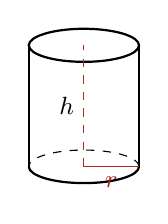
\begin{tikzpicture}[scale=0.7,font=\small]
\draw[thick] (-1,0) arc (180:360:1 and 0.3); \draw[dashed] (1,0) arc (0:180:1 and 0.3);
\draw[thick] (0,2.2) ellipse (1 and 0.3); \draw[thick] (-1,0)--(-1,2.2); \draw[thick] (1,0)--(1,2.2);
\draw[cThm] (0,0)--(1,0) node[midway,below]{$r$}; \draw[cThm,dashed] (0,0)--(0,2.2); \node[left] at (0,1.1){$h$};
\end{tikzpicture}\end{LTR}}
\newcommand{\ConeFig}{\begin{LTR}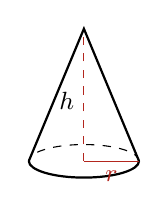
\begin{tikzpicture}[scale=0.7,font=\small]
\draw[thick] (-1,0) arc (180:360:1 and 0.3); \draw[dashed] (1,0) arc (0:180:1 and 0.3);
\draw[thick] (-1,0)--(0,2.4)--(1,0);
\draw[cThm] (0,0)--(1,0) node[midway,below]{$r$}; \draw[cThm,dashed] (0,0)--(0,2.4); \node[left] at (0,1.1){$h$};
\end{tikzpicture}\end{LTR}}
\newcommand{\SphFig}{\begin{LTR}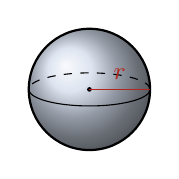
\begin{tikzpicture}[scale=0.7,font=\small]
\shade[ball color=cDef!20] (0,0) circle (1.1); \draw[thick] (0,0) circle (1.1);
\draw (-1.1,0) arc (180:360:1.1 and 0.3); \draw[dashed] (1.1,0) arc (0:180:1.1 and 0.3);
\fill (0,0) circle (1.2pt); \draw[cThm] (0,0)--(1.1,0) node[midway,above]{$r$};
\end{tikzpicture}\end{LTR}}
% هرم رباعي SABCD قاعدته مربع ومركزها O
\newcommand{\PyrFig}[1]{\begin{LTR}\begin{tikzpicture}[scale=#1,font=\small,line join=round]
\coordinate (A) at (0,0); \coordinate (B) at (2.4,0); \coordinate (C) at (3.3,0.9); \coordinate (D) at (0.9,0.9);
\coordinate (O) at (1.65,0.45); \coordinate (S) at (1.65,2.8); \coordinate (I) at ($(B)!0.5!(C)$);
\draw[thick] (A)--(B)--(C); \draw[dashed] (C)--(D)--(A); \draw[thick] (S)--(A); \draw[thick] (S)--(B); \draw[thick] (S)--(C); \draw[dashed] (S)--(D);
\draw[dashed,cThm] (S)--(O); \draw[dashed] (A)--(C); \draw[dashed] (B)--(D); \draw[cRem] (S)--(I);
\foreach \p/\pos in {A/below left,B/below right,C/right,D/left,S/above,O/below,I/right} \node[\pos] at (\p){$\p$};
\end{tikzpicture}\end{LTR}}
\SetHeader{\small\bfseries\color{cSec}ملخص: الهندسة في الفضاء}{\small\color{cSec}السنة الأولى ثانوي -- جذع مشترك علوم وتكنولوجيا}
\begin{document}
\begin{LTR}
\begin{tcolorbox}[enhanced,colback=cSec!10,colframe=cSec!40,arc=3mm,halign=center,boxrule=0.6pt,top=12pt,bottom=12pt,before upper={\selectlanguage{arabic}}]
{\color{cSec}\fontsize{28}{34}\selectfont\bfseries الهندسة في الفضاء}\\[8pt]
{\color{cSec!80!black}\large ملخص شامل مع أشكال وأمثلة وتمارين محلولة خطوة بخطوة}\\[5pt]
{\color{cSec!80!black}\large السنة الأولى ثانوي -- جذع مشترك علوم وتكنولوجيا}
\end{tcolorbox}
\end{LTR}

\begin{BOX}{cSec}{محتوى الملخص}
\begin{multicols}{2}
\begin{enumerate}[label=\textbf{\arabic*.}]
\item المجسمات المألوفة: الأطوال والمساحات والحجوم.
\item التصميم والمنظور متساوي القياس.
\item الموضوعات الأولية في الفضاء.
\item الأوضاع النسبية لمستقيمين.
\item الأوضاع النسبية لمستقيم ومستوٍ.
\item الأوضاع النسبية لمستويين.
\item التوازي في الفضاء.
\item التعامد في الفضاء وحساب الأطوال.
\item تمارين محلولة.
\item خلاصة الطرائق.
\end{enumerate}
\end{multicols}
\end{BOX}

% =====================================================================
\section{المجسمات المألوفة: الأطوال والمساحات والحجوم}
\begin{tarif}[المجسمات المألوفة]
\begin{itemize}
\item \textbf{متوازي المستطيلات:} مجسم له ستة أوجه كلها مستطيلات ، أبعاده: الطول $a$ ، العرض $b$ ، الارتفاع $c$.
\item \textbf{المكعب:} متوازي مستطيلات أوجهه الستة مربعات متقايسة طول حرفها $a$.
\item \textbf{الموشور القائم:} قاعدتان مضلعان متقايسان في مستويين متوازيين ، وأوجه جانبية مستطيلات.
\item \textbf{الهرم:} قاعدته مضلع ، وأوجهه الجانبية مثلثات لها رأس مشترك $S$ (رأس الهرم).
\item \textbf{الأسطوانة القائمة والمخروط والكرة:} مجسمات دورانية ، $r$ نصف القطر و $h$ الارتفاع.
\end{itemize}
\end{tarif}

\begin{LTR}\begin{center}
\begin{tabular}{ccccc}
\BoxFig{2}{1.6}{1.3}{0.9} & \CylFig & \ConeFig & \SphFig & \PyrFig{0.65}\\[2pt]
\ar{متوازي مستطيلات} & \ar{أسطوانة} & \ar{مخروط} & \ar{كرة} & \ar{هرم}
\end{tabular}
\end{center}\end{LTR}

\begin{khassia}[دساتير المساحات والحجوم]
\begin{center}
\renewcommand{\arraystretch}{1.7}
\begin{tabular}{|>{\centering\arraybackslash}p{0.27\textwidth}|>{\centering\arraybackslash}p{0.36\textwidth}|>{\centering\arraybackslash}p{0.22\textwidth}|}
\hline\rowcolor{cSec!12}
\textbf{الحجم $V$} & \textbf{المساحة} & \textbf{المجسم}\\\hline
$a^3$ & $6a^2$ & المكعب (حرفه $a$)\\\hline
$abc$ & $2(ab+bc+ca)$ & متوازي المستطيلات\\\hline
$\mathcal B\times h$ & الجانبية: محيط القاعدة $\times\, h$ & الموشور القائم\\\hline
$\pi r^2h$ & الجانبية: $2\pi rh$ ، الكلية: $2\pi rh+2\pi r^2$ & الأسطوانة القائمة\\\hline
$\dfrac13\,\mathcal B\times h$ & مجموع مساحات الأوجه & الهرم\\\hline
$\dfrac13\,\pi r^2h$ & -- & المخروط الدوراني\\\hline
$\dfrac43\,\pi r^3$ & $4\pi r^2$ & الكرة\\\hline
\end{tabular}
\end{center}
حيث $\mathcal B$ مساحة القاعدة و $h$ الارتفاع.
\end{khassia}

\begin{molahada}[الوحدات]
\begin{itemize}
\item الأطوال بـ $\mathrm{cm}$ ، المساحات بـ $\mathrm{cm}^2$ ، الحجوم بـ $\mathrm{cm}^3$.
\item \LW{$1\,\mathrm{L}=1\,\mathrm{dm}^3=1000\,\mathrm{cm}^3$} \quad و \quad \LW{$1\,\mathrm{m}^3=1000\,\mathrm{L}$}.
\item نوحّد الوحدات دائمًا قبل الحساب.
\end{itemize}
\end{molahada}

\begin{mithal}
\begin{itemize}
\item أسطوانة نصف قطرها $3\,\mathrm{cm}$ وارتفاعها $10\,\mathrm{cm}$:\quad $V=\pi\times3^2\times10=\bx{90\pi\approx282{,}7\ \mathrm{cm}^3}$.
\item كرة نصف قطرها $6\,\mathrm{cm}$:\quad $V=\dfrac43\pi\times6^3=\bx{288\pi\ \mathrm{cm}^3}$ \quad و \quad $\mathcal A=4\pi\times36=\bx{144\pi\ \mathrm{cm}^2}$.
\item هرم قاعدته مربع ضلعه $6\,\mathrm{cm}$ وارتفاعه $4\,\mathrm{cm}$:\quad $V=\dfrac13\times36\times4=\bx{48\ \mathrm{cm}^3}$.
\end{itemize}
\end{mithal}

% =====================================================================
\section{التصميم والمنظور متساوي القياس}
\begin{tarif}[التصميم]
\textbf{تصميم} مجسم هو شكل مستوٍ نحصل عليه بفرد سطح المجسم (فتحه وبسطه على مستوٍ) ، ويسمح بصنع المجسم بالطي.
\end{tarif}

\RL{0.5}{%
\begin{mithal}[تصميم مكعب]
تصميم المكعب: ستة مربعات متقايسة مرتبة بحيث لا يتراكب أي وجهين عند الطي.\par
تصميم الأسطوانة: مستطيل بعداه $2\pi r$ و $h$ ، وقرصان نصف قطر كل منهما $r$.
\end{mithal}}{0.46}{%
\begin{LTR}\begin{center}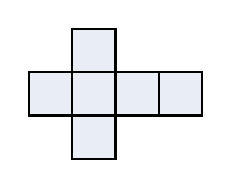
\begin{tikzpicture}[scale=0.55]
\foreach \x/\y in {1/0,0/1,1/1,2/1,3/1,1/2} \draw[thick,fill=cDef!10] (\x,\y) rectangle ++(1,1);
\end{tikzpicture}\end{center}\end{LTR}}

\begin{khassia}[قواعد المنظور متساوي القياس]
\begin{itemize}
\item الوجه الأمامي (والوجوه الموازية له) يُرسم بأبعاده الحقيقية.
\item الأحرف العمودية على الوجه الأمامي تُرسم مائلة وبطول مُصغَّر.
\item المستقيمات المتوازية تُرسم متوازية ، ويُحافَظ على منتصف قطعة.
\item الأحرف المخفية تُرسم بخطوط متقطعة.
\end{itemize}
\end{khassia}

\begin{molahada}
في المنظور متساوي القياس \textbf{لا تُحفَظ} كل الأطوال ولا كل الزوايا القائمة: الوجه $BCGF$ للمكعب مربع ، لكنه يُرسم متوازي أضلاع.
\end{molahada}

% =====================================================================
\section{الموضوعات الأولية في الفضاء}
\begin{khassia}[موضوعات]
\begin{enumerate}
\item من نقطتين متمايزتين يمر \textbf{مستقيم وحيد}.
\item من ثلاث نقط ليست على استقامة واحدة يمر \textbf{مستوٍ وحيد}.
\item إذا شمل مستوٍ نقطتين متمايزتين $A$ و $B$ فإنه يشمل كل نقط المستقيم $(AB)$.
\item كل مبرهنات الهندسة المستوية صحيحة في كل مستوٍ من الفضاء.
\end{enumerate}
\end{khassia}

\begin{molahada}[تعيين مستوٍ]
يتعيّن مستوٍ بإحدى المعطيات: ثلاث نقط ليست على استقامة واحدة ، أو مستقيم ونقطة خارجه ، أو مستقيمين متقاطعين ، أو مستقيمين متوازيين تمامًا.
\end{molahada}

% =====================================================================
\section{الأوضاع النسبية لمستقيمين}
\begin{khassia}
لمستقيمين $(d)$ و $(d')$ في الفضاء حالتان:
\begin{itemize}
\item \textbf{من نفس المستوي:} إما متقاطعان في نقطة وحيدة ، وإما متوازيان (تمامًا أو منطبقان).
\item \textbf{ليسا من نفس المستوي:} لا يتقاطعان ولا يتوازيان.
\end{itemize}
\end{khassia}

\RL{0.55}{%
\begin{mithal}[في المكعب $ABCDEFGH$]
\begin{itemize}
\item $(AB)$ و $(HG)$: \bxt{متوازيان} (الرباعي $ABGH$ مستطيل).
\item $(AB)$ و $(BF)$: \bxt{متقاطعان في $B$}.
\item $(AE)$ و $(BC)$: \bxt{ليسا من نفس المستوي}.
\item $(AG)$ و $(EC)$: \bxt{متقاطعان} (قطرا المستطيل $ACGE$).
\end{itemize}
\end{mithal}}{0.4}{%
\begin{center}\CubeFig{0.9}{\draw[cThm,thick] (A)--(G); \draw[cThm,thick] (E)--(C);}\end{center}}

\begin{molahada}
في الفضاء: مستقيمان لا يتقاطعان \textbf{ليسا بالضرورة متوازيين}.
\end{molahada}

% =====================================================================
\section{الأوضاع النسبية لمستقيم ومستوٍ}
\begin{khassia}
لمستقيم $(d)$ ومستوٍ $(P)$ ثلاث حالات:
\begin{itemize}
\item $(d)$ \textbf{محتوى} في $(P)$: كل نقط $(d)$ من $(P)$.
\item $(d)$ \textbf{يوازي} $(P)$ تمامًا: لا نقطة مشتركة بينهما.
\item $(d)$ \textbf{يقطع} $(P)$ في نقطة وحيدة.
\end{itemize}
\end{khassia}

\begin{LTR}\begin{center}
\begin{tabular}{ccc}
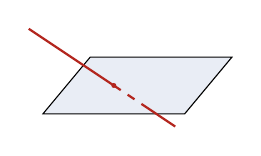
\begin{tikzpicture}[scale=0.6]
\draw[fill=cDef!10] (0,0)--(3,0)--(4,1.2)--(1,1.2)--cycle; \draw[cThm,thick] (-0.3,1.8)--(1.5,0.6); \fill[cThm] (1.5,0.6) circle(1.5pt);
\draw[cThm,thick,dashed] (1.5,0.6)--(2.1,0.2); \draw[cThm,thick] (2.1,0.2)--(2.8,-0.27);
\end{tikzpicture} &
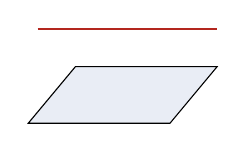
\begin{tikzpicture}[scale=0.6]
\draw[fill=cDef!10] (0,0)--(3,0)--(4,1.2)--(1,1.2)--cycle; \draw[cThm,thick] (0.2,2)--(4,2);
\end{tikzpicture} &
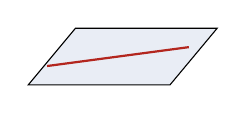
\begin{tikzpicture}[scale=0.6]
\draw[fill=cDef!10] (0,0)--(3,0)--(4,1.2)--(1,1.2)--cycle; \draw[cThm,thick] (0.4,0.4)--(3.4,0.8);
\end{tikzpicture}\\
\ar{يقطعه في نقطة} & \ar{يوازيه تمامًا} & \ar{محتوى فيه}
\end{tabular}
\end{center}\end{LTR}

\begin{mithal}[في المكعب $ABCDEFGH$]
$(AB)$ محتوى في $(ABCD)$ ؛ \quad $(EF)$ يوازي $(ABCD)$ تمامًا ؛ \quad $(AE)$ يقطع $(ABCD)$ في $A$.
\end{mithal}

% =====================================================================
\section{الأوضاع النسبية لمستويين}
\begin{khassia}
لمستويين $(P)$ و $(Q)$ حالتان:
\begin{itemize}
\item \textbf{متوازيان:} متوازيان تمامًا (لا نقطة مشتركة) أو منطبقان.
\item \textbf{متقاطعان:} تقاطعهما مستقيم.
\end{itemize}
\end{khassia}

\begin{mithal}[في المكعب $ABCDEFGH$]
\begin{itemize}
\item $(ABCD)$ و $(EFGH)$: \bxt{متوازيان تمامًا}.
\item $(ABFE)$ و $(BCGF)$: \bxt{متقاطعان وفق المستقيم $(BF)$}.
\end{itemize}
\end{mithal}

\begin{tariqa}[إيجاد تقاطع مستويين]
نبحث عن \textbf{نقطتين مشتركتين} بين المستويين: المستقيم الذي يشملهما هو تقاطع المستويين.
\end{tariqa}

% =====================================================================
\section{التوازي في الفضاء}
\begin{khassia}[مبرهنات التوازي]
\begin{enumerate}
\item إذا وازى مستقيمان مستقيمًا ثالثًا فإنهما متوازيان.
\item يوازي مستقيم مستويًا إذا وازى مستقيمًا من هذا المستوي.
\item يتوازى مستويان إذا وازى مستقيمان متقاطعان من أحدهما المستوي الآخر.
\item إذا توازى مستويان فإن كل مستوٍ يقطع أحدهما يقطع الآخر ، والمستقيمان الناتجان متوازيان.
\end{enumerate}
\end{khassia}

\begin{mithal}
في المكعب: $(EG)\parallel(AC)$ لأن $ACGE$ مستطيل ، و $(AC)$ محتوى في $(ABCD)$ ، إذن \bxt{$(EG)$ يوازي المستوي $(ABCD)$}.
\end{mithal}

\begin{molahada}
مستقيم يوازي مستويًا \textbf{لا يوازي بالضرورة} كل مستقيمات هذا المستوي: $(EF)$ يوازي $(ABCD)$ لكنه لا يوازي $(BC)$.
\end{molahada}

% =====================================================================
\section{التعامد في الفضاء وحساب الأطوال}
\begin{khassia}[التعامد]
\begin{enumerate}
\item يكون مستقيم \textbf{عموديًا على مستوٍ} إذا عامد \textbf{مستقيمين متقاطعين} من هذا المستوي.
\item إذا كان مستقيم عموديًا على مستوٍ فإنه يعامد \textbf{كل} مستقيمات هذا المستوي.
\item مستقيمان عموديان على نفس المستوي متوازيان.
\end{enumerate}
\end{khassia}

\RL{0.55}{%
\begin{mithal}[قطر المكعب]
مكعب طول حرفه $a$:
\begin{itemize}
\item في المربع $ABCD$: $AC^2=a^2+a^2$ ، إذن $AC=a\sqrt2$.
\item $(CG)$ يعامد $(CB)$ و $(CD)$ المتقاطعين ، فهو عمودي على $(ABCD)$ ، إذن $(CG)\perp(AC)$.
\item المثلث $ACG$ قائم في $C$: $AG^2=2a^2+a^2=3a^2$ ، إذن \bx{AG=a\sqrt3}.
\end{itemize}
\end{mithal}}{0.4}{%
\begin{center}\CubeFig{0.9}{\draw[cThm,thick] (A)--(G); \draw[cDef,thick,dashed] (A)--(C); \draw[cDef,thick] (C)--(G);}\end{center}}

\begin{khassia}[قطر متوازي المستطيلات]
قطر متوازي مستطيلات أبعاده $a$ ، $b$ ، $c$ هو \quad \LW{$d=\sqrt{a^2+b^2+c^2}$}.
\end{khassia}

\begin{tariqa}[حساب طول في مجسم]
نبحث عن \textbf{مثلث قائم} في مستوٍ مناسب يكون الطول المطلوب أحد أضلاعه ، ونبرر الزاوية القائمة بالتعامد بين مستقيم ومستوٍ ، ثم نطبق مبرهنة فيثاغورس.
\end{tariqa}

% =====================================================================
\section{تمارين محلولة}
\begin{tmr}
متوازي مستطيلات أبعاده $3\,\mathrm{cm}$ ، $4\,\mathrm{cm}$ و $12\,\mathrm{cm}$.
\begin{enumerate}
\item احسب مساحته الكلية وحجمه.
\item احسب طول قطر قاعدته ($3\times4$) ، ثم طول قطره.
\end{enumerate}
\end{tmr}
\begin{hal}
\QQ{1} $\mathcal A=2(3\times4+4\times12+12\times3)=2(12+48+36)=\bx{192\ \mathrm{cm}^2}$ \quad ؛ \quad $V=3\times4\times12=\bx{144\ \mathrm{cm}^3}$.
\QQ{2} قطر القاعدة: $\sqrt{3^2+4^2}=\sqrt{25}=\bx{5\ \mathrm{cm}}$.\par
الحرف الذي طوله $12$ عمودي على القاعدة ، فالمثلث المكوَّن قائم: $d=\sqrt{5^2+12^2}=\sqrt{169}=\bx{13\ \mathrm{cm}}$.
\end{hal}

\begin{tmr}
مجسم مكوَّن من مكعب طول حرفه $6\,\mathrm{cm}$ ، يعلوه هرم قاعدته الوجه العلوي للمكعب وارتفاعه $4\,\mathrm{cm}$.
\begin{enumerate}
\item احسب حجم المجسم.
\item احسب الارتفاع $SI$ لوجه جانبي للهرم ($I$ منتصف حرف القاعدة) ، ثم المساحة الكلية للمجسم.
\end{enumerate}
\end{tmr}
\begin{hal}
\QQ{1} $V=6^3+\dfrac13\times6^2\times4=216+48=\bx{264\ \mathrm{cm}^3}$.
\QQ{2} مركز القاعدة $O$ يبعد عن منتصف الحرف بـ $3$ ، و $(SO)$ عمودي على القاعدة ، فالمثلث $SOI$ قائم في $O$:\par
$SI=\sqrt{4^2+3^2}=\bx{5\ \mathrm{cm}}$.\par
المساحة الكلية = خمسة أوجه للمكعب + أربعة مثلثات: $5\times36+4\times\dfrac{6\times5}2=180+60=\bx{240\ \mathrm{cm}^2}$.
\end{hal}

\begin{tmr}
$ABCDEFGH$ مكعب. عيّن الوضع النسبي في كل حالة مع التبرير:
\begin{enumerate}
\item المستقيمان $(EG)$ و $(AC)$.
\item المستقيم $(FH)$ والمستوي $(ABC)$.
\item المستويان $(ACGE)$ و $(BDHF)$.
\end{enumerate}
\end{tmr}
\begin{hal}
\QQ{1} $AE=CG$ و $(AE)\parallel(CG)$ ، إذن $ACGE$ متوازي أضلاع (بل مستطيل) ، ومنه \bxt{$(EG)\parallel(AC)$}.
\QQ{2} بنفس الطريقة $(FH)\parallel(BD)$ ، و $(BD)$ محتوى في $(ABC)$ ، و $(FH)$ لا يشمل أي نقطة من $(ABC)$: \bxt{$(FH)$ يوازي $(ABC)$ تمامًا}.
\QQ{3} ليكن $O$ مركز $ABCD$ و $O'$ مركز $EFGH$. النقطة $O$ تنتمي إلى $(AC)$ و $(BD)$ فهي مشتركة بين المستويين ، وكذلك $O'$. إذن \bxt{المستويان متقاطعان وفق المستقيم $(OO')$}.
\end{hal}

% =====================================================================
\section{خلاصة الطرائق}
\begin{center}
\renewcommand{\arraystretch}{1.5}
\begin{tabular}{|p{0.62\textwidth}|p{0.3\textwidth}|}
\hline\rowcolor{cSec!12}
\textbf{الطريقة} & \textbf{المطلوب}\\\hline
نختار الدستور المناسب ، ونوحّد الوحدات ($1\,\mathrm{L}=1\,\mathrm{dm}^3$). & حساب حجم أو مساحة\\\hline
نجد مثلثًا قائمًا في مستوٍ مناسب ونطبق فيثاغورس. & حساب طول في مجسم\\\hline
نثبت أنهما يوازيان مستقيمًا ثالثًا ، أو أنهما ضلعان متقابلان في متوازي أضلاع. & إثبات توازي مستقيمين\\\hline
نثبت أنه يوازي مستقيمًا من هذا المستوي. & إثبات توازي مستقيم ومستوٍ\\\hline
نثبت أن مستقيمين متقاطعين من أحدهما يوازيان الآخر. & إثبات توازي مستويين\\\hline
نجد نقطتين مشتركتين بينهما. & تعيين تقاطع مستويين\\\hline
نثبت أنه يعامد مستقيمين متقاطعين من المستوي. & إثبات تعامد مستقيم ومستوٍ\\\hline
\end{tabular}
\end{center}
\end{document}
